\documentclass[11pt]{article}

\usepackage[left=0.75in, right=0.75in, top=0.75in, bottom=0.75in]{geometry}
\usepackage{layout}
\usepackage{ucs}
\usepackage[utf8x]{inputenc}
\usepackage{titlesec}
\usepackage{graphicx}
\usepackage{amssymb}
\usepackage{amsmath}
\usepackage{dsfont}
\usepackage{float}
\usepackage{caption}
\usepackage{subcaption}
\usepackage{array}



\title{\textbf{TS114 Project}\\Computer-aided analysis of electrocardiogram signals}
\author{Maxime PETERLIN - \texttt{maxime.peterlin@enseirb-matmeca.fr}\\
Gabriel VERMEULEN - \texttt{gabriel@vermeulen.email} \\\\{ENSEIRB-MATMECA, Bordeaux}}
\date{June, 6th 2014}


\begin{document}

\maketitle
\tableofcontents

\newpage

\section{Introduction}
	The heart has always been an accurate indicator of one's health. Analyzing it and monitoring its activity is of utmost importance for clinicians. Thus this project's aim is to develop an automatic and user-friendly application capable of giving useful information about heart activity, such as cardiac rhythm or detection of heart conditions, based on an electrocardiogram signal.\\\\
	The project is divided into multiple parts. First, different ECG signals (from both ill and healthy people) were displayed and analysed under MATLAB to highlight their characteristics. Subsequently, the automated detection of the latter was implemented, as well as the identification of cardiac pathologies and the ECG signals denoising. Finally, the ultimate product is delivered with a Graphical User Interface (GUI) making it possible for the clinicians to use it easily and intuitively.\\


\section{ECG visualization}
	In this first part, seven different ECG signals will be analyzed and displayed under MATLAB. \\Three of these are records from healthy patients' heart, whereas the other four are from ill ones, each with different pathologies.\\
	This part's aim is to study these signals in the frequency and time domain, starting by the latter, and underline the different characteristics and properties of these.

	\subsection{Time display}
		\begin{figure}[ht]
			\centering
			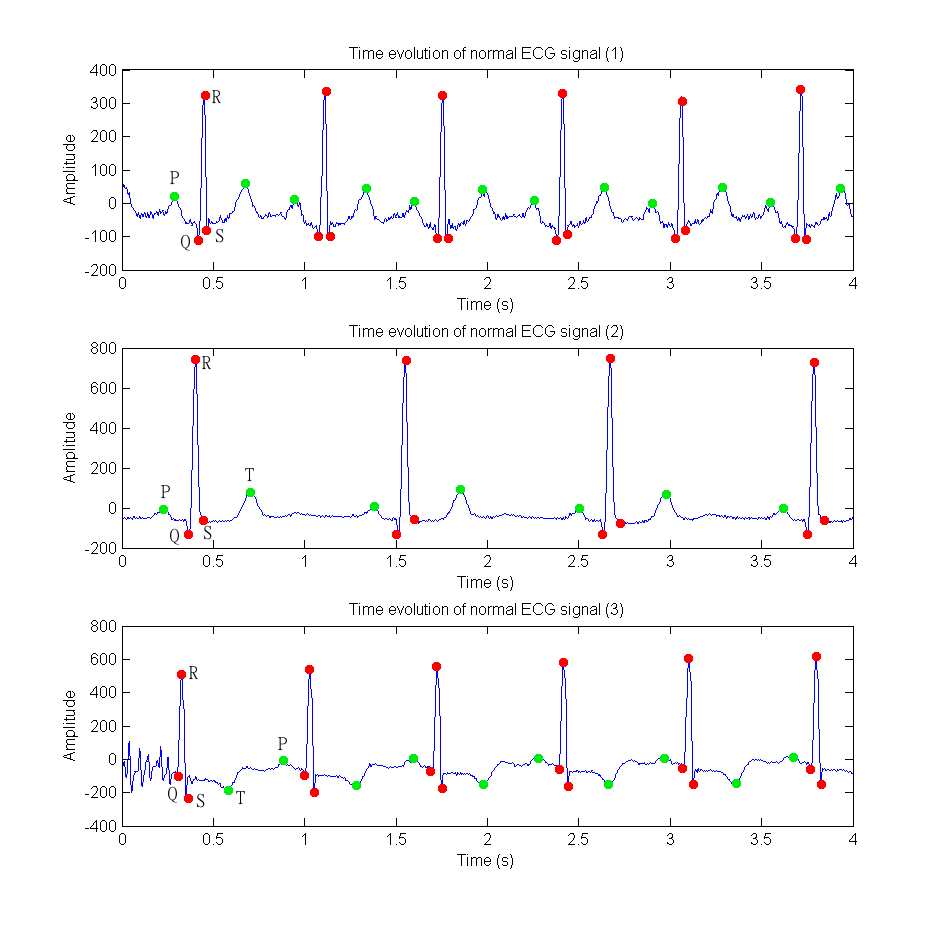
\includegraphics[scale=0.65]{images/Q311.png}
			\caption{Normal ECG signals with the Q, R, S points and P, T waves highlighted}
			\label{Q311}
		\end{figure}

		First, three seconds of each of the aforementioned normal ECG signals (i.e. from healthy hearts) were plotted under MATLAB. On the figure above (Figure~\ref{Q311}), their Q, R and S points are represented by red dots, while their P and T waves are located by green dots.  \\
		\\
		The first signal displayed is noisier than the other two, although, its characteristic points and waves are easier to observe.\\
		The second signal is uncluttered, but the S points are hardly recognizable.\\
		Finally, the P and T waves of the third signal, which is slightly noisy, are nearly overlapping.\
		\\
		Based on these four second samples, the cardiac rhythm of each patient was computed and displayed in the table below.\\
		\begin{center}
			\begin{tabular}{|c|c|c|}
				\hline
				\textbf{Signal number} & \textbf{Cardiac rhythm (bpm)} \\
				\hline
				1 & 91.7 \\ 
				\hline
				2 & 53.0 \\
				\hline
				3 & 86.4 \\
				\hline
			\end{tabular}
		\end{center}
		\vspace{0.3in}
		According to the graphs and the computed cardiac rhythms, it can be assumed that the faster the heartbeat is, the noisier the ECG will be.\\
		Moreover, the second signal represents the ECG of a heart with a slow heartbeat and since it is a normal ECG, it might be the heartbeat of an athletic person (otherwise it could be a heart condition like bradycardia).\\
		\\
		\begin{figure}[ht]
			\centering
			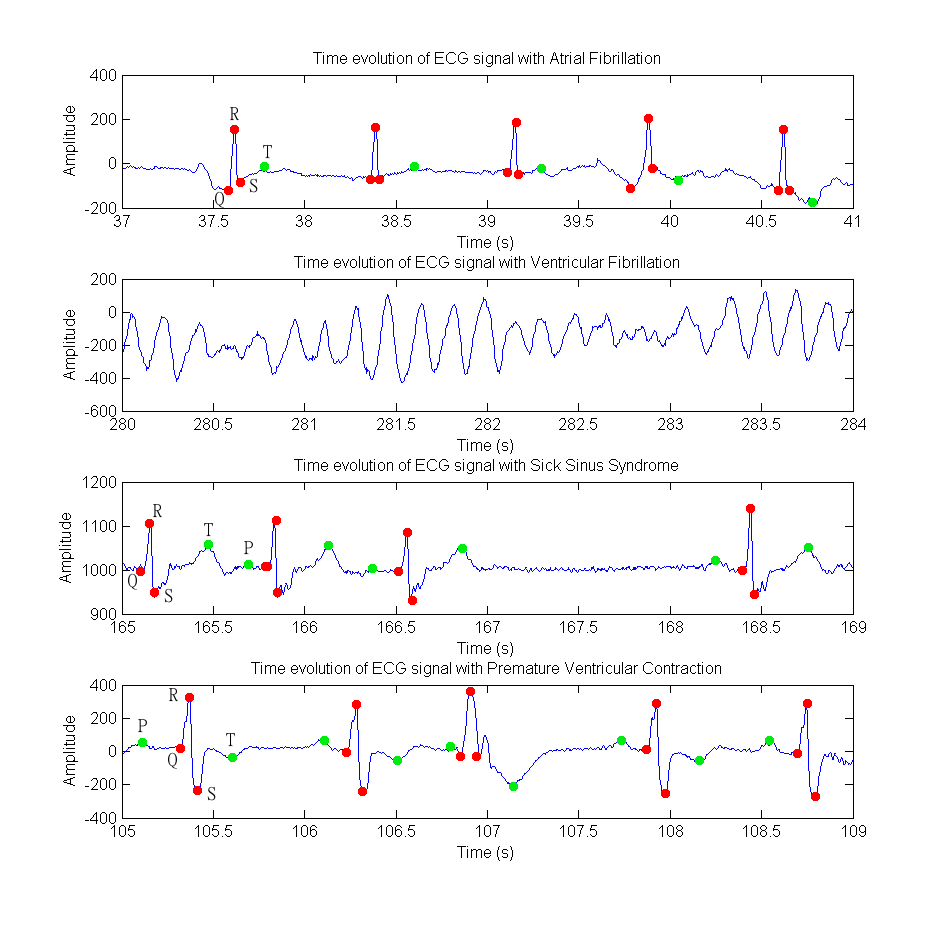
\includegraphics[scale=0.65]{images/Q312.png}
			\caption{ECG signals with pathologies with the Q, R, S points and P, T waves highlighted}
			\label{Q312}
		\end{figure}
		\\
		Then, the last four ECG signals associated with heart conditions were plotted under MATLAB.\\
		The corresponding cardiac rhythms were computed and displayed in the table below.\\ 
		\begin{center}
			\begin{tabular}{|c|c|c|}
				\hline
				\textbf{Pathology} & \textbf{Cardiac rhythm (bpm)} \\
				\hline
				Atrial Fibrillation & 76.7 \\ 
				\hline
				Ventricular Fibrillation & 55.5 \\
				\hline
				Sick Sinus Syndrome & 84.7 \\
				\hline
				Premature Ventricular Contraction & 71.1 \\
				\hline
			\end{tabular}
		\end{center}
		\vspace{0.3in}
		These pathologies have an impact on each ECG signal and useful characteristics are lost.\\
		Compared to the normal signals, the Atrial Fibrillation's ECG signals lack P waves and has weak impulsions. Similarly, for the Ventricular Fibrillation, the signal depicts a fast heartbeat and hardly discernible P, Q, R, S and T waves.\\
		The Sick Sinus Syndrome has a different effect on the signal, for it creates groups of P waves and R/S points with an absence of activity in between.\\
		The Premature Ventricular Contraction pathology is the closest match, out of the four signals, to a typical one. But, as the pathology's name suggests, the P waves are ahead compared to a normal signal.\\

	\subsection{Frequency display}
		At first, the ECG power spectrum of the normal ECG signals. $N$ samples were used, with $N = 15 \cdot F_s$.\\
		\\
		\begin{figure}[ht]
			\centering
			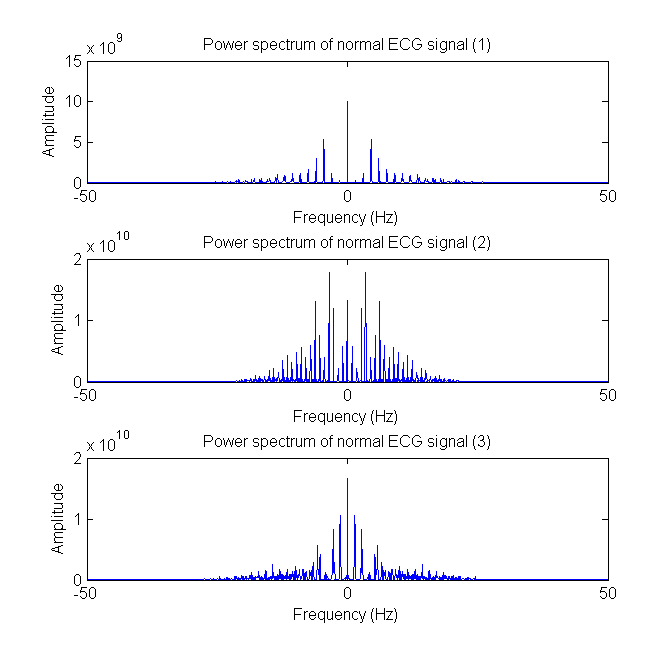
\includegraphics[scale=0.65]{images/Q321.png}
			\caption{ECG power spectrum of the normal ECG signals}
			\label{Q321}
		\end{figure}
		\\
		Since the original signals are periodic, peaks can be found every $f = \frac{n}{T_b}, \forall n \in \mathbb{N}$.\\
		$T_b$ represents the number of beats per second. It is then possible to compute the different cardiac rhythms which are shown in the table below.\\
		\begin{center}
			\begin{tabular}{|c|c|c|}
				\hline
				\textbf{Signal number} & \textbf{Cardiac rhythm (bpm)} \\
				\hline
				1 & 91.8 \\ 
				\hline
				2 & 52.2 \\
				\hline
				3 & 81.9 \\
				\hline
			\end{tabular}
		\end{center}
		\vspace{0.3in}
		The results are quite close to what was computed in the time domain.\\
		\\
		Then, the signals associated with pathologies were plotted under MATLAB.\\
		\\
		\begin{figure}[ht]
			\centering
			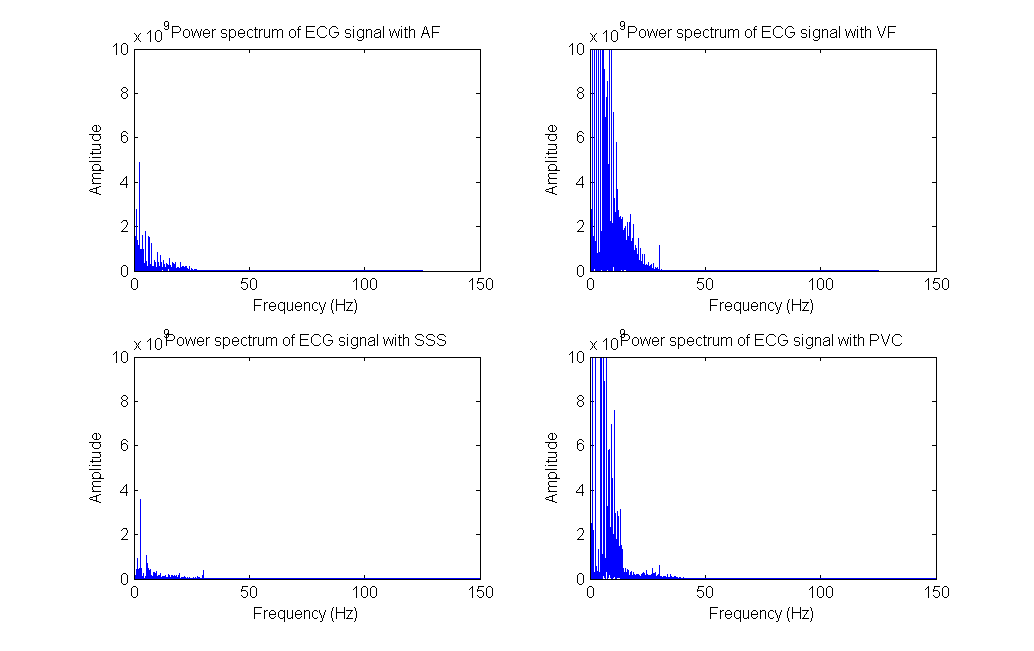
\includegraphics[scale=0.65]{images/Q322.png}
			\caption{ECG power spectrum of the ECG signals associated with pathologies}
			\label{Q322}
		\end{figure}
		\\
		These graphs were cut off, otherwise, since the component in $f = 0$ has a very high value, the scale follows suit and it is almost impossible to see the other components.\\
		The differences between these power spectra and those from the normal ECG, are firstly, as it was said above, the value of the $f=0$ component.\\
		It can also be noted that these power spectra are not as clear and organized as the first ones, indeed, it is harder to point out and see the different peaks.
		\\
		Out of the previous results, the cardiac rhythms were computed and displayed in the table below. 
		\begin{center}
			\begin{tabular}{|c|c|c|}
				\hline
				\textbf{Pathology} & \textbf{Cardiac rhythm (bpm)} \\
				\hline
				Atrial Fibrillation & 76.8 \\ 
				\hline
				Ventricular Fibrillation & 57.6 \\
				\hline
				Sick Sinus Syndrome & 82.8 \\
				\hline
				Premature Ventricular Contraction & 72 \\
				\hline
			\end{tabular}
		\end{center}
		\vspace{0.3in}
		Just as before, the results match those computed in the time domain.



\section{Detection of P, QRS and T waves}
	\subsection{Three different methods of R waves detection}
		The purpose of this section is to implement and compare three different methods in order to detect the R waves.
		\subsubsection{Method of local maxima}
			\begin{figure}[ht]
				\centering
				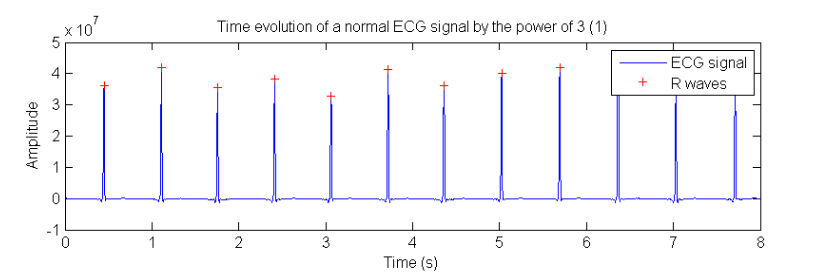
\includegraphics[scale=0.5]{images/Q411_lm.png}
				\caption{Normal ECG by the power of 3}
				\label{Q411_lm}
			\end{figure}
			This method is rather straightforward. A window is set to work on a restricted number of samples. The signal is then cubed to make the R waves stand out.\\
			A threshold $r$ is chosen to only select the peaks corresponding to the R waves. $r$ is a variable equal to a certain percentage of the maximum value contained in the ECG signals.\\
			When the peaks are picked, the local maxima of the latter is selected and the corresponding times taken out. Finally, the R points are plotted on the original ECG at the previously found positions.\\
			This method is pretty successful in general, however, if the different R waves' amplitude vary greatly, or if the amplitude of P and T waves amplitude are as high as R waves, detection errors might occur.
		\subsubsection{Method of the derivative}
			\begin{figure}[ht]
				\centering
				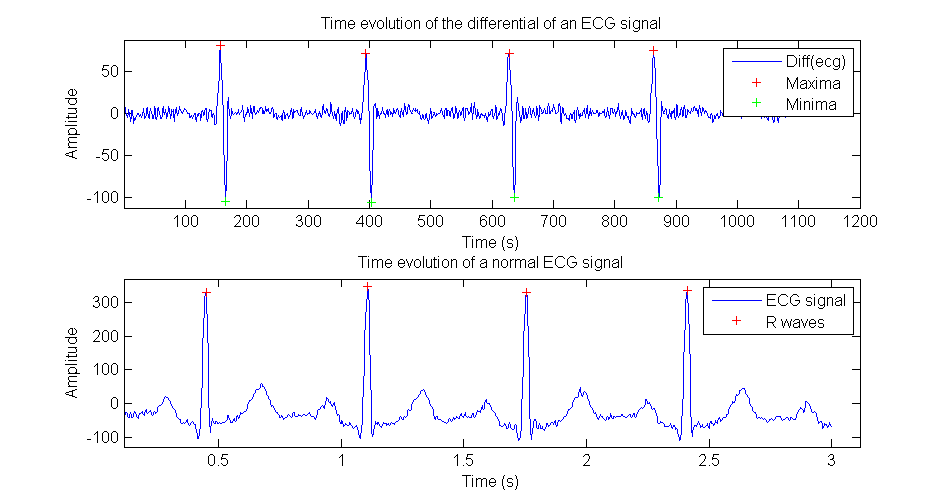
\includegraphics[scale=0.5]{images/Q411_d.png}
				\caption{Time evolution of an ECG signal and its differential}
				\label{Q411_d}
			\end{figure}
			The derived ECG signals presents peaks with a local maxima followed by a local minima. Using the previous method, these different peaks are located with their beginning and ending times. The latter is transposed to the original ECG signals to get the different R waves domains. The R points correspond to the local maximum in each given domain.\\
			On the one hand, compared to the previous method, this one can successfully detect R waves with different amplitudes. On the other hand, there are globally more mistakes and issues with this method than the other, especially on certain ECG signals with high variations.\\
		\subsubsection{Pan and Tompkins algorithm}
			\begin{figure}[h]
				\centering
				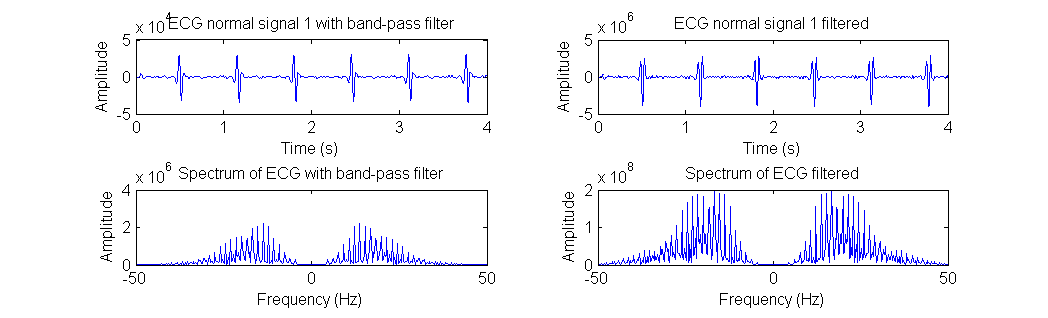
\includegraphics[scale=0.5]{images/Q411_pt_2.png}
				\caption{ECG signal filtered by a band-pass filter}
				\label{Q411_pt_2}
			\end{figure}
			As opposed to the previous methods, the Pan and Tompkins algorithm consists of different steps.\\
			First, the ECG signal is filtered by a band-pass filter, which is composed of a low pass-filter and a high pass-filter.\\
			The resulting signal is filtered by a derivative signal to gain information about the QRS slope and then squared to make the local maxima stand out.\\
			\begin{figure}[h]
				\centering
				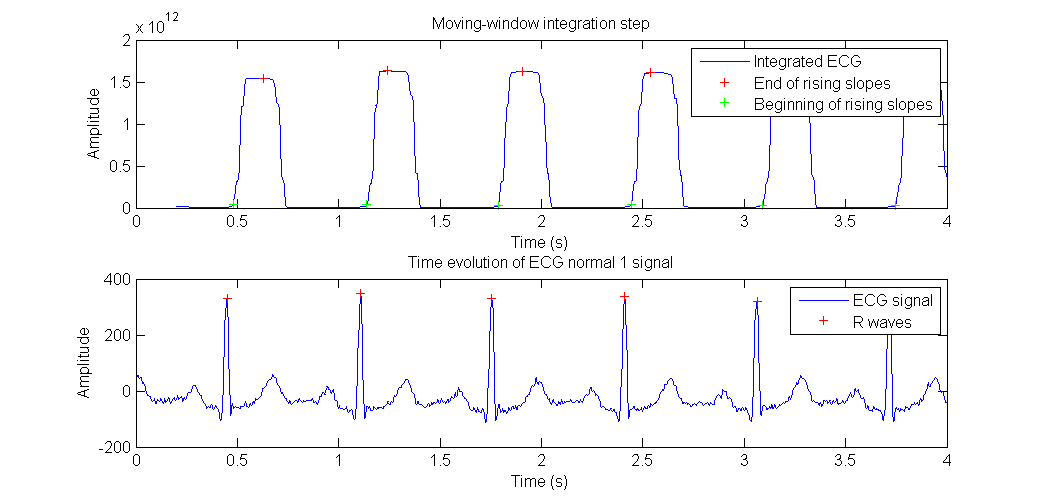
\includegraphics[scale=0.5]{images/Q411_pt_4.png}
				\caption{Moving-window integration step}
				\label{Q411_pt_4}
			\end{figure}
			\\
			Then, the signal is integrated with a moving-window method. The width of the said window is $N = 0.2 s$ which is the empirically-determined duration of a QRS complex.\\
			Finally, a threshold is applied on the integrated signal. Thanks to this step, the temporal location of the QRS complex can be extracted from the rising slope in the latter.
			This method is the most efficient of them all, it can almost always detect the R waves perfectly. Although, errors might occur on some specific ECGs, these could originate from the signal integration with the detection of the rising slope.\\
	\subsection{Q and S waves detection}
		Based on the R waves' location, it is now possible to detect the Q and S waves. They are respectively defined as the first minima preceding and following the R waves.\\
		This definition is unfortunately too plain to be effective. If the signal happens to be slightly noisy, another minimum could be detected between the R wave and the actual Q or S wave. A solution could be the addition of a thresholding step to make sure that the amplitude between the R wave and the eventual Q or S waves is higher than a given level.
	\subsection{P and T waves detection}
		At first, the ECG signal is filtered with a low-pass filter to remove the noise and make it smoother. It is then filtered by a differentiator, exactly like the R waves detection, to identify the local maxima and thus point out the P and T waves.\\
		Although, if the ECG is too noisy, it is hard to detect efficiently the zero crossing point, but the error is negligible.\\
			\begin{figure}[h]
				\centering
				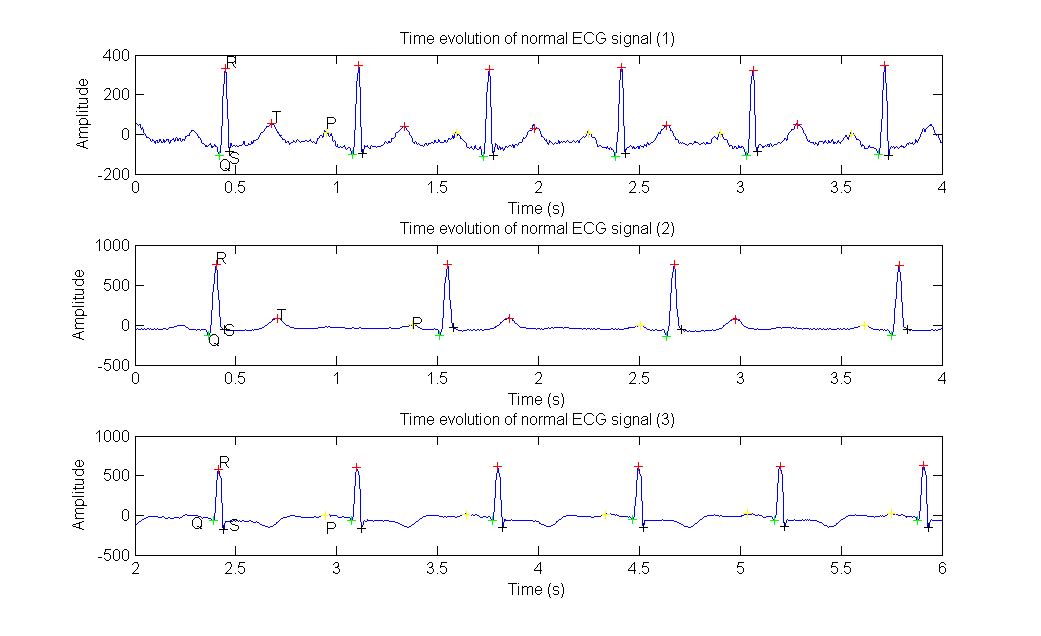
\includegraphics[scale=0.5]{images/Q42_4.png}
				\caption{P, Q, R, S and T waves detection}
				\label{Q412}
			\end{figure}


\section{Automatic identification of cardiac pathologies}
	Now that the P, Q, R, S and T waves detection has been achieved, it can be put to a practical use. Indeed, in the following part, different pathologies identification methods will be studied and implemented.
	\subsection{Tachycardia/Bradycardia}
		The cardiac rhythm has been defined as the time between two R waves. Tachycardia (respectively bradycardia) is declared when the former is over 100 bpm (respectively under 60 bpm).\\
		A simple method was used to compute the cardiac rhythm. At first, 4 seconds of the given ECG are isolated, the R waves are then detected and the time between them computed. All these times are summed and then divided by the number of R-R intervals to obtain an average time between the different R waves. The cardiac rhythm is finally computed based on the previous result. \\
		Identifying basic arrhythmia pathologies now boils down to a simple comparison between the cardiac rhythm and the threshold defining these pathologies (60 bpm and 100 bpm in this case).\\
		\\
		It was suggested to use the entire ECG to compute the cardiac rhythm, but it is a quite clumsy approach. Indeed, the heartbeat can vary greatly, especially for ill people. It seemed more logical to use small samples temporally speaking, to have a more representative quantification of the cardiac rhythm.\\
		It also unveils the main problem of the sample mean method. The cardiac rhythm cannot be precisely estimated, because it is subject to change throughout the ECG signal. It is only an average value and the solution would be, as it was done above, to use samples temporally restricted and compute the rhythm on a given window.
		I can also be noted that this method is highly dependent on the R waves detection. Thus, the latter must be as precise as possible.
	\subsection{Heart rate variability}
		The heart rate variability $v$ can be used to detect pathologies such as myocardial dysfunction and it is the linear interpolation between two subsequent R-R intervals' value.\\
		The power spectrum of $v$ actually needs a huge amount of samples to be representative and the resulting spectrum is still tainted by a cardinal sine.\\
		For an adult, the respiratory rhythm usually ranges between 12 and 20 cycles per minute. It corresponds respectively to a frequency of 0.2 Hz and 0.33 Hz. Therefore, the respiratory oscillations can be detected in the high frequency band.
	\subsection{Ectopic beat}
		A heartbeat is said to be ectopic if, at a given time, the next R waves occurs earlier than expected and is followed by a longer R-R interval until the next normal beat.\\
		A threshold $\epsilon$ equal to 5 bpm is used to detect these premature beats. The results are excellent if the R waves detection is spot-on.
	\subsection{Atrial Fibrillation}
		When atrial fibrillation occurs, the temporal difference between each R waves (the process $(\Delta_n)_{n \ge 0}$ ) can be modeled as a white noise. Thus, an interesting manner to detect if whether the studied ECG segment presents an atrial fibrillation or not is to compute the autocovariance function of $(\Delta_n)_{n \ge 0}$.\\
		Also, during atrial fibrillation, the P waves are absent, which is an easier way to detect or justify the presence of an illness.
	\subsection{Ventricular Fibrillation}
		Ventricular fibrillations are basically a sine wave with fast oscillations : about 200 bpm to 600 bpm.\\
		Based on this definition two approaches were used. The first one consisted in computing the cardiac rhythm, but in order to detect the pathology, the peaks detection needed to be perfect which was not the case.\\
		The other possible method was a spectral approach. The fast heartbeat component can be found and isolated in the power spectrum of the ECG signal.

		
\section{ECG denoising}
	Baseline wander, power line interference or muscle activities can be the cause of the noises tainting the ECG signals. To prevent the loss of useful information, the signal must be filtered upfront. \\
	This section is aimed at getting rid of the baseline as well as the 50 Hz power line interferences polluting the ECG signals.\\
	On the power spectrum, the power line component appears distinctly (a peak when $f=50 Hz$) and can be taken care of using a low-pass filter. The temporal results are satisfying since the signal appears to be cleaned off.\\
	Electrodes malfunction can cause baseline wandering, where the signal seems to be moving up and down. A high-pass filter can be used to get rid of the effect and, based on the post-filtering results, in a successful manner.


\section{Graphical User Interface}

\section{Conclusion}
	This project and its practical application to the medical field highlighted the importance and the main concepts behind numeric signal processing. ECG analysis is compulsory to establish a diagnosis, therefore it is of utmost importance to easily and rapidly have access to the principal data that can be extracted from these ECG signals, especially when every second is a matter of life and death.\\
	Thus, based on different ECG signals and the extrapolation of their data, we were able to create an automatic detection of different cardiac pathologies and display the most important information into a user-friendly Graphical User Interface (GUI).\\
	Finally, this assignment gave us a better understanding of what an ECG is and how to process it as well as technical knowledge on numeric signal processing passing through the use of Matlab.\\

\end{document}
